% !TEX program = xelatex
\documentclass[11pt,a4paper]{article}

\usepackage{polyglossia}
\setdefaultlanguage{french}
\usepackage{fontspec}
\usepackage{amsmath,amssymb}
\usepackage[margin=2.3cm]{geometry}
\usepackage{graphicx}
\usepackage{subcaption}
\usepackage{booktabs}
\usepackage{tikz}
\usetikzlibrary{arrows.meta,calc}
\usepackage{xcolor}
\usepackage{enumitem}
\usepackage[hidelinks]{hyperref}

\definecolor{tronbleu}{RGB}{25,190,255}
\definecolor{cluorange}{RGB}{255,115,20}

\setlist{itemsep=2pt,topsep=4pt}
\newcommand{\pos}[1]{\left(#1\right)_+}
\newcommand{\code}[1]{\texttt{#1}}

\title{\textbf{TRON 3D --- Light Cycles}\\[2pt]\large Ce que le jeu doit au cours d'INF443}
\author{Philibert Pappens\\\small Projet réalisé avec Wandrille Boivin --- École polytechnique, INF443}
\date{Octobre 2026}

\begin{document}
\maketitle

\noindent Jeu de motos de lumière en 3D, en C++/OpenGL avec la bibliothèque CGP du cours. Il tourne sur PC et dans le navigateur (WebAssembly), et se joue sur téléphone en l'inclinant comme un volant.

\noindent Code : \url{https://github.com/PhilibertPap/tron}\\
Jeu en ligne : \url{https://philibertpap.github.io/tron/}

Ce document reprend chaque brique du jeu et la relie aux notions du cours : transformations, maillages, illumination, textures, animation physique, collisions.

\begin{figure}[h]
	\centering
	\begin{subfigure}{0.49\linewidth}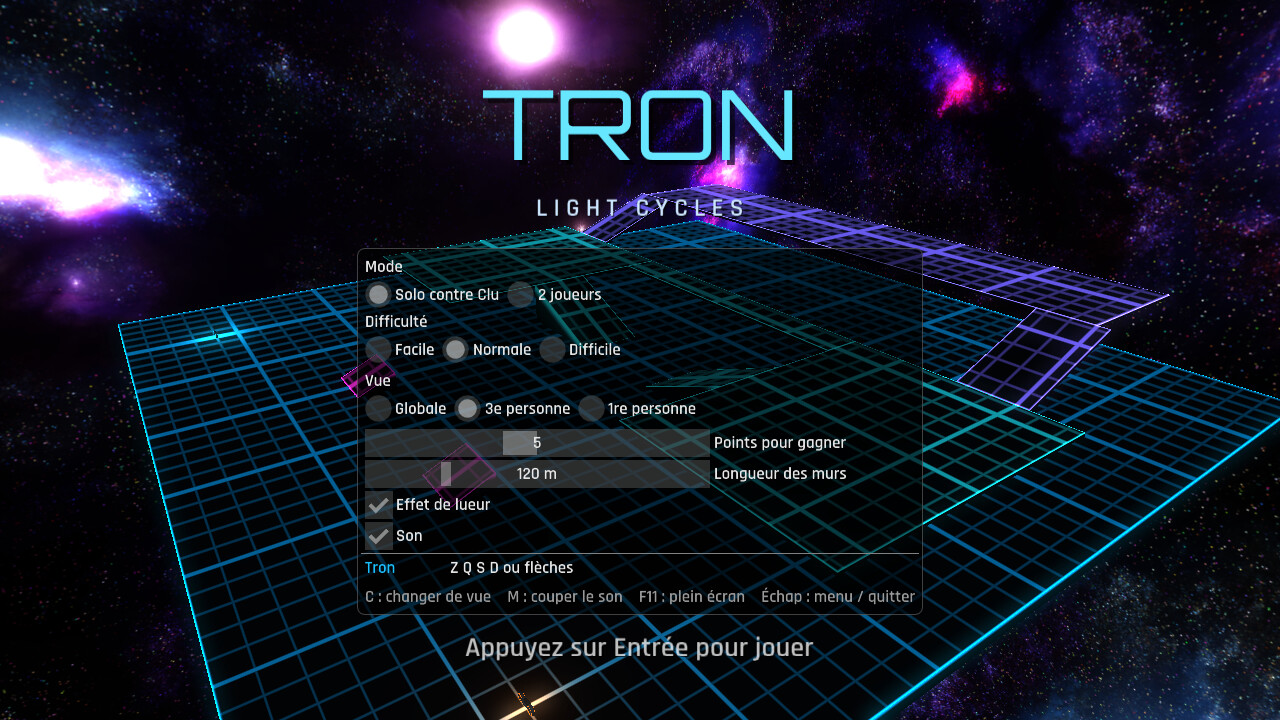
\includegraphics[width=\linewidth]{figures/titre.jpg}\caption{Écran titre}\end{subfigure}\hfill
	\begin{subfigure}{0.49\linewidth}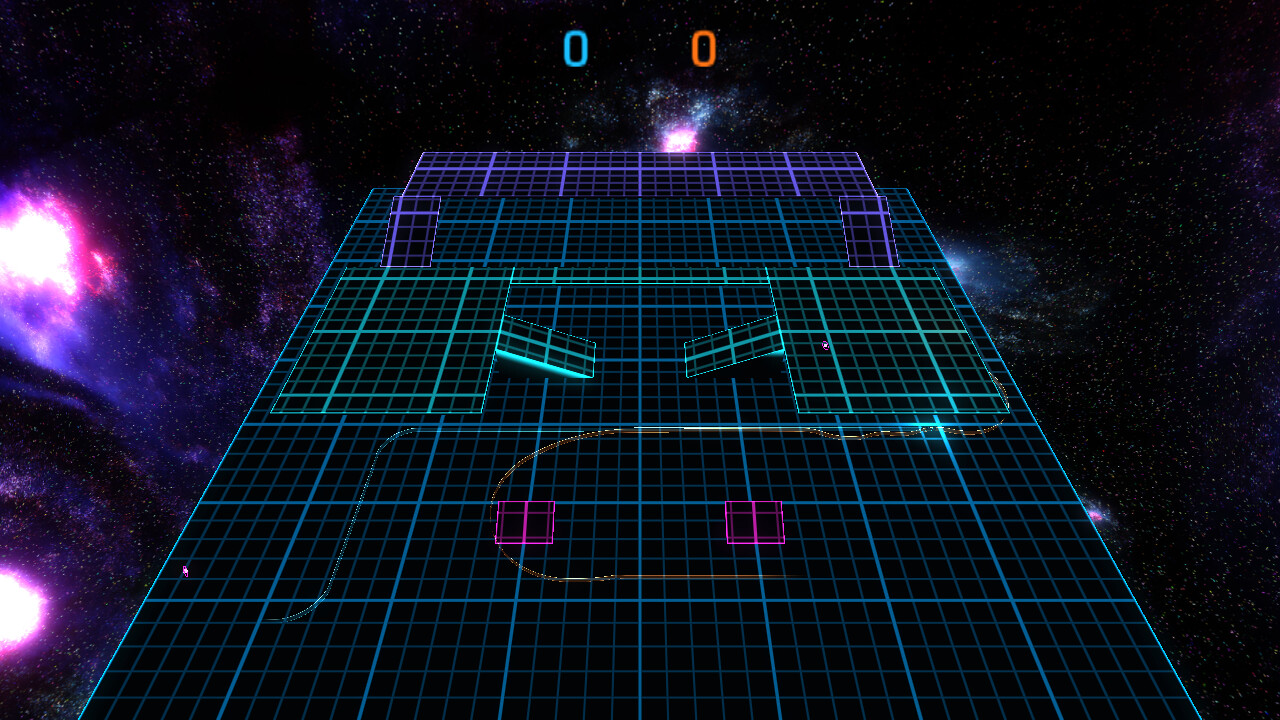
\includegraphics[width=\linewidth]{figures/arene.jpg}\caption{Arène vue de haut : sol, étages, rampes, tremplins}\end{subfigure}
	\caption{Tron (bleu) contre Clu (orange, piloté par l'IA en solo).}
\end{figure}

% ---------------------------------------------------------------------------
\section{Architecture}

\begin{itemize}
	\item Boucle de jeu : à chaque image, \code{update(dt)} puis \code{render()} ; $dt$ est borné à $0{,}05$~s pour éviter les sauts après une image lente.
	\item Machine à états : écran titre $\to$ compte à rebours $\to$ manche $\to$ fin de manche $\to$ fin de partie.
	\item Les commandes sont séparées de la physique : une moto reçoit seulement $(a, \sigma) \in [-1,1]^2$ (accélérateur, braquage), produits par le clavier, l'IA ou le téléphone.
\end{itemize}

% ---------------------------------------------------------------------------
\section{Transformations et repères}

\paragraph{Coordonnées homogènes.} Toutes les transformations sont des matrices $4\times4$ agissant sur $(x,y,z,1)$ :
$M = \begin{pmatrix} R & t \\ 0 & 1 \end{pmatrix}$. Comme dans le cours, la matrice la plus à droite est appliquée en premier.

\paragraph{Modèle hiérarchique de la moto} (cours §5.4, solides articulés). Arbre de transformations
\[
	M_{\text{monde}}(\text{roue}) = \underbrace{T(p)\,R_z(\psi)\,R_y(\theta)}_{\text{moto}}\;\underbrace{R_x(-\varphi)}_{\text{châssis}}\;\underbrace{T(\pm x_r, 0, z_r)}_{\text{roue}}
\]
avec $\psi$ le cap, $\theta$ le tangage et $\varphi$ l'inclinaison dans les virages.
\begin{itemize}
	\item Tangage : le nez suit la vitesse, $\theta = \operatorname{atan2}(-v_z, v_h)$ (montée de rampe, saut, chute).
	\item Inclinaison : $\varphi \leftarrow \varphi + \min(1, k\,dt)\,(\sigma\varphi_{\max} - \varphi)$, avec $\varphi_{\max} = 0{,}45$~rad.
	\item Normales : $N_{\text{monde}} = (M^{-1})^{T} N$, calculée une fois par objet côté CPU plutôt qu'à chaque sommet dans le shader.
\end{itemize}

\paragraph{Caméras.} Matrice de vue $V = F^{-1}$, où $F$ est le repère « look-at » construit à partir de l'œil $e$, de la cible $c$ et de la verticale $e_z$. Trois vues :
\begin{itemize}
	\item globale : caméra orbitale du cours, pilotée à la souris ;
	\item 3\textsuperscript{e} personne : $e^\star = p - 7f + 3e_z$, $c^\star = p + 5f$ (avec $f$ la direction de la moto) ;
	\item 1\textsuperscript{re} personne : œil juste devant le phare.
\end{itemize}
La caméra suit sa cible avec un retard, $e \leftarrow e + \min(1, k\,dt)\,(e^\star - e)$ : c'est le schéma d'Euler de $\dot e = k(e^\star - e)$, dont la solution exponentielle a pour constante de temps $1/k \approx 0{,}17$~s.

% ---------------------------------------------------------------------------
\section{Maillages}

\paragraph{Mur de lumière.} Le tracé est une suite de points $p_0, \dots, p_n$ espacés d'au moins $\delta = 0{,}5$~m, plus la tête $h$, collée à l'arrière de la moto. Le mur est une bande de triangles (fig.~\ref{fig:bande}) :
\[
	v_{2k} = p_k,\qquad v_{2k+1} = p_k + H e_z,\qquad \text{triangles } (2k,\,2k{+}2,\,2k{+}1),\ (2k{+}1,\,2k{+}2,\,2k{+}3).
\]
\begin{itemize}
	\item Le maillage est alloué une seule fois pour $N_{\max} = L_{\max}/\delta + 8$ points. Les sommets inutilisés sont ramenés sur la tête : leurs triangles sont dégénérés (aire nulle) et ne produisent aucun pixel. À chaque image, on ne fait que réécrire les positions dans le buffer existant. La première version recréait tous les buffers à chaque image, ce qui provoquait une fuite de mémoire GPU.
	\item La longueur est limitée en mètres : on retire des points en queue tant que $\sum \lVert p_{k+1} - p_k \rVert > L$. Avant, on comptait les points, et le mur était deux fois plus court à 120 images/s qu'à 60.
	\item Coordonnée de texture $u = s/S$ (abscisse curviligne normalisée), utilisée pour estomper la queue du mur.
\end{itemize}

\begin{figure}[h]
	\centering
	\begin{tikzpicture}[scale=1.15]
		\foreach \i/\x/\y in {0/0/0, 1/1.4/0.25, 2/2.8/0.2, 3/4.2/-0.15, 4/5.6/-0.6} {
			\coordinate (b\i) at (\x,\y);
			\coordinate (t\i) at (\x,\y+1.2);
		}
		\foreach \i/\j in {0/1, 1/2, 2/3, 3/4} {
			\fill[tronbleu!25] (b\i) -- (b\j) -- (t\j) -- (t\i) -- cycle;
			\draw[tronbleu!70] (b\i) -- (t\j);
		}
		\draw[tronbleu, thick] (b0) -- (b1) -- (b2) -- (b3) -- (b4);
		\draw[tronbleu, very thick] (t0) -- (t1) -- (t2) -- (t3) -- (t4);
		\foreach \i in {0,...,4} { \draw[tronbleu!70] (b\i) -- (t\i); \fill (b\i) circle (1.3pt); }
		\node[below] at (b0) {$v_0 = p_0$}; \node[above] at (t0) {$v_1$};
		\node[below] at (b1) {$v_2$}; \node[above] at (t1) {$v_3$};
		\node[below right] at (b4) {$h$ (tête)};
		\draw[-{Stealth}] (6.3,-0.6) -- (7.4,-0.6) node[right] {moto};
		\draw[{Stealth}-{Stealth}] (-0.4,0) -- (-0.4,1.2) node[midway,left] {$H$};
	\end{tikzpicture}
	\caption{Le mur de lumière comme bande de triangles le long du tracé.}
	\label{fig:bande}
\end{figure}

\paragraph{Niveau.} Chaque surface (sol, étage, rampe, tremplin) a une emprise rectangulaire $[a_x, b_x]\times[a_y, b_y]$ et une altitude affine le long d'un axe $i$ :
\[
	z(p) = z_a + \frac{p_i - a_i}{b_i - a_i}\,(z_b - z_a).
\]
Les étages sont des dalles fines (on peut rouler dessous), les rampes des volumes pleins. Le maillage de chaque surface se compose du dessus, des flancs et, pour les dalles, du dessous. La moto est faite de primitives du cours (ellipsoïdes, tores).

% ---------------------------------------------------------------------------
\section{Illumination}

Modèle de Phong du cours (éq.~2.1) :
\[
	I = (C : I_a) + \sum_{s\in S} \Big[ k_d \pos{L_s\cdot N}\,(C : I_s) + k_s \pos{R_s\cdot V}^{n} I_s \Big].
\]
\begin{itemize}
	\item Les sources : chaque moto est une lumière ponctuelle de sa couleur (elle éclaire le sol et l'autre moto), plus une lumière d'appoint directionnelle.
	\item Atténuation des sources ponctuelles : $I_s \leftarrow f(d_s)\, I_s$ avec $f(d) = 1/(1 + a d + b d^2)$, $a = 0{,}08$, $b = 0{,}03$.
	\item Objets lumineux (bandes de la moto, murs, bonus) : $k_a = 1$, $k_d = k_s = 0$, d'où $I = C$.
	\item Un bug de la première version s'explique par le produit terme à terme : une lumière cyan $(0,1,1)$ appliquée à une moto jaune $(1,1,0)$ donne $(0,1,1):(1,1,0) = (0,1,0)$, du vert.
\end{itemize}

% ---------------------------------------------------------------------------
\section{Texture procédurale et aliassage}

La grille du sol était au départ une texture image. Vue en incidence rasante, elle scintillait : c'est l'aliassage du cours (§4.5). Elle est maintenant calculée dans le fragment shader à partir de la position $x$ (en cellules) :
\[
	d(x) = \left|\operatorname{fract}\!\left(x - \tfrac12\right) - \tfrac12\right|, \qquad
	w = \left|\frac{\partial x}{\partial X}\right| + \left|\frac{\partial x}{\partial Y}\right|, \qquad
	\text{ligne} = 1 - \operatorname{clamp}\!\left(\frac{d}{w} - \frac{\lambda}{2},\,0,\,1\right).
\]
\begin{itemize}
	\item $d$ est la distance à la ligne la plus proche, et $w$ (\code{fwidth} en GLSL) la variation de $x$ d'un pixel à l'autre de l'écran. Le rapport $d/w$ est donc une distance en pixels.
	\item Les lignes ont la même largeur $\lambda$ en pixels quelle que soit la distance, avec un bord adouci d'un pixel. C'est un préfiltrage analytique, l'équivalent du choix de niveau de mipmap du cours, mais exact.
\end{itemize}

% ---------------------------------------------------------------------------
\section{Transparence et post-traitement}

\paragraph{Murs transparents.} Mélange additif $C_{\text{écran}} \leftarrow C_{\text{écran}} + \alpha\, C_{\text{mur}}$, avec les murs dessinés en dernier sans écrire dans le z-buffer. L'addition étant commutative, il n'y a pas besoin de trier les murs par profondeur.

\paragraph{Lueur (bloom).} Quatre passes sur des textures hors écran :
\begin{enumerate}
	\item rendu de la scène dans une texture ;
	\item extraction des zones lumineuses, $w = \operatorname{clamp}\big((\max(r,g,b) - s)/(1 - s), 0, 1\big)$ avec $s = 0{,}55$ ;
	\item flou gaussien séparable à demi-résolution : $G(x,y) = g(x)\,g(y)$, donc deux passes 1D de 9 échantillons au lieu de 81. Trois itérations, et les variances s'ajoutent : $\sigma_{\text{tot}} = \sqrt{3}\,\sigma$ ;
	\item composition : $I = I_{\text{scène}} + \beta\, I_{\text{halo}}$.
\end{enumerate}

\begin{figure}[h]
	\centering
	\begin{subfigure}{0.49\linewidth}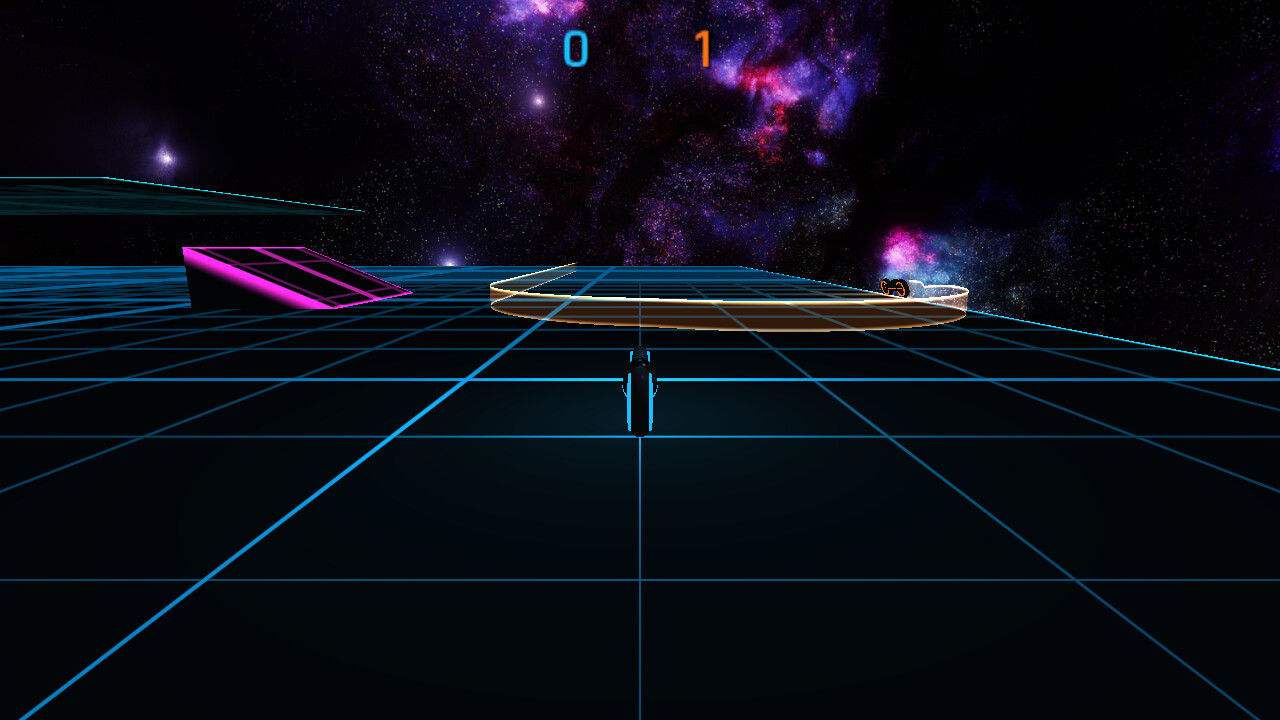
\includegraphics[width=\linewidth]{figures/course_sans_bloom.jpg}\caption{Sans lueur}\end{subfigure}\hfill
	\begin{subfigure}{0.49\linewidth}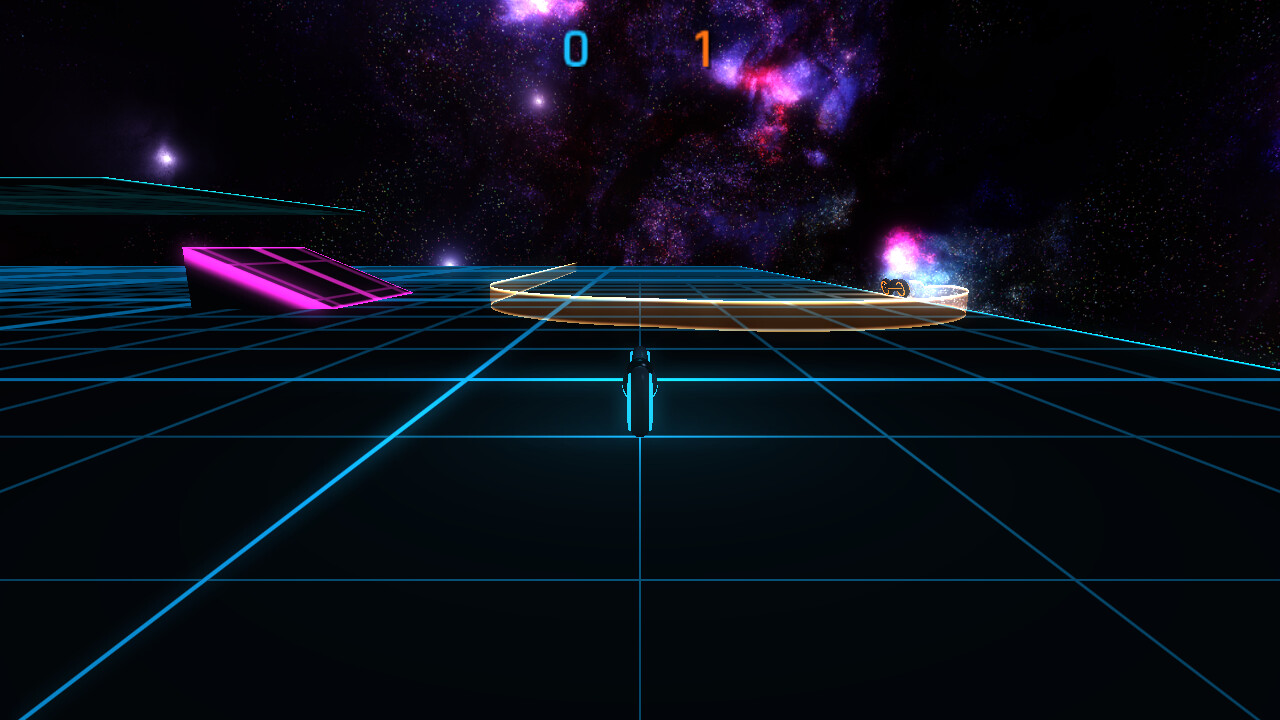
\includegraphics[width=\linewidth]{figures/course.jpg}\caption{Avec lueur}\end{subfigure}
	\caption{Même image, avec et sans le post-traitement : le mur de Clu forme une boucle devant Tron.}
\end{figure}

% ---------------------------------------------------------------------------
\section{Animation physique}

\paragraph{Mouvement horizontal.} Le joueur choisit une vitesse visée $v^\star \in \{9, 18, 28\}$~m/s ($42$ en boost), que la moto rejoint au premier ordre :
\[
	v \leftarrow v + \min(1, k\,dt)\,(v^\star - v), \qquad \psi \leftarrow \psi + \sigma\,\omega\,dt,
\]
d'où un rayon de virage $R = v/\omega \approx 7$~m à $18$~m/s ($\omega = 2{,}6$~rad/s). Freiner permet donc de tourner plus serré.

\paragraph{Vertical : Euler semi-implicite} (comme la boucle d'animation du cours, §6.2.2) :
\[
	v_z \leftarrow v_z - g\,dt, \qquad z \leftarrow z + v_z\,dt \quad (\text{avec la \emph{nouvelle} vitesse}),\qquad g = 25~\text{m/s}^2.
\]
\begin{itemize}
	\item Hauteur du sol sous $p$ : $h(p) = \max\{z_s(p) : z_s(p) \le z + \Delta\}$ parmi les surfaces qui contiennent $p$, avec $\Delta = 0{,}6$~m. On ne monte pas sur un étage situé au-dessus de soi.
	\item Au sol, la moto suit le relief : $z = h$ et $v_z = (h - z)/dt$ (vitesse de montée sur une rampe).
	\item Quand le sol se dérobe (bout de tremplin, bord d'étage), la moto garde ce $v_z$ et part en vol libre. Sur un tremplin de pente $\tan\alpha = 3/7$ à $18$~m/s, $v_z \approx 7{,}7$~m/s, soit $\Delta z = v_z^2/2g \approx 1{,}2$~m au-dessus du tremplin.
	\item Sous l'altitude $-4$~m, la moto est perdue dans le vide.
\end{itemize}

\paragraph{Particules} (cours §6.4). L'explosion est un système de 160 particules : vitesse initiale aléatoire sur la demi-sphère, gravité, frottement de l'air $v \leftarrow (1 - c\,dt)\,v$, durée de vie limitée.

% ---------------------------------------------------------------------------
\section{Détection des collisions}

Le cours le souligne (§6.3.1) : à pas de temps discret, les collisions sont détectées trop tard. Ici, le problème était l'effet tunnel. La première version testait si la moto était à moins de $0{,}6$~m d'un point du mur, alors qu'en boost elle avance de $42/60 = 0{,}7$~m par image : elle pouvait traverser un mur sans le toucher.

\paragraph{Test balayé.} On teste le segment parcouru par l'avant de la moto pendant $dt$, $[a, b]$ avec $r = b - a$, contre chaque segment du mur $[p, q]$ avec $s = q - p$. On résout $a + t\,r = p + u\,s$ à l'aide du produit vectoriel 2D $x \times y = x_1 y_2 - x_2 y_1$ :
\[
	t = \frac{(p - a)\times s}{r \times s}, \qquad u = \frac{(p - a)\times r}{r \times s}, \qquad \text{croisement} \iff t, u \in [0, 1] \quad (r\times s \neq 0).
\]
\paragraph{Passage en 3D.} En cas de croisement vu de dessus, on compare les hauteurs au point d'intersection :
\[
	z_m = z_a + t\,(z_b - z_a), \quad z_w = z_p + u\,(z_q - z_p), \qquad
	\text{choc} \iff [z_m,\, z_m + h_m] \cap [z_w,\, z_w + H] \neq \varnothing.
\]
On peut donc passer sous un mur posé à l'étage, ou sauter par-dessus.
\begin{itemize}
	\item Son propre mur : on ignore les deux derniers segments, collés à la roue arrière.
	\item Décor : choc si l'avant de la moto entre dans le volume d'une surface, entre son dessous et son dessus moins $\Delta$ (flanc de rampe, bord d'étage).
	\item Les chocs sont d'abord tous relevés, puis appliqués : deux motos qui s'écrasent à la même image font égalité.
	\item Coût : $O(N)$ par moto, $N \approx 240$ segments. La grille de détection large du cours n'est pas nécessaire ici ; elle le deviendrait avec beaucoup de motos ou des murs infinis.
\end{itemize}

\begin{figure}[h]
	\centering
	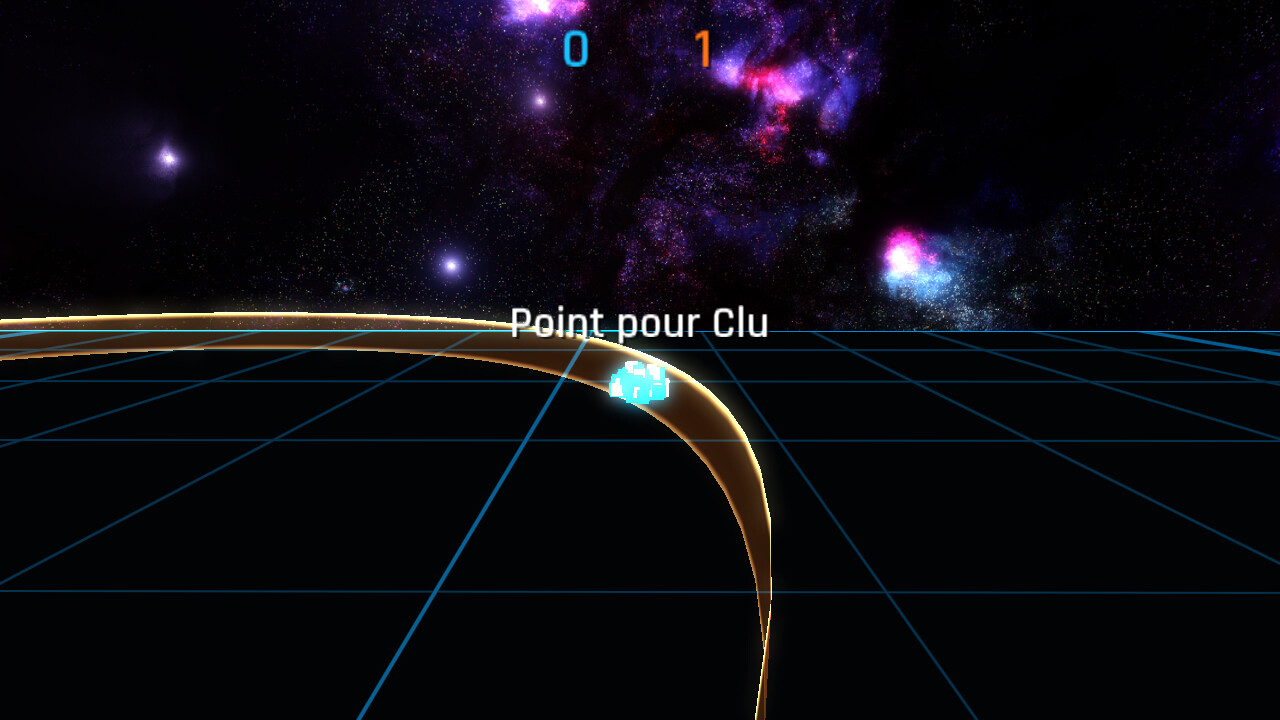
\includegraphics[width=0.6\linewidth]{figures/crash.jpg}
	\caption{Tron percute le mur de Clu : explosion de particules.}
\end{figure}

% ---------------------------------------------------------------------------
\section{Intelligence artificielle}

Clu choisit son braquage par simulation. Plusieurs fois par seconde, pour chaque braquage candidat $\sigma \in \{0, \pm0{,}35, \pm0{,}7, \pm1\}$ :
\begin{enumerate}
	\item on simule la trajectoire, un arc de cercle de courbure $\kappa = \sigma\omega/v$, par pas de 1~m sur une distance d'anticipation $L$ ;
	\item à chaque pas, mêmes tests que pour les vraies collisions (murs, décor, vide), plus le trajet probable de l'adversaire pendant la seconde suivante ;
	\item $d(\sigma)$ est la distance parcourue avant le premier obstacle (au plus $L$).
\end{enumerate}
On garde $\sigma^\star = \arg\max J(\sigma)$, avec
\[
	J(\sigma) = d(\sigma) + \mathbf{1}_{d(\sigma) = L}\,\big(15\,\gamma\, B_{\text{adv}} + 10\, B_{\text{boost}}\big) - 1{,}5\,|\sigma| + 0{,}5\;\mathbf{1}_{\sigma = \sigma_{\text{préc}}},
\]
où $B_{\text{adv}}, B_{\text{boost}} \in [0,1]$ valent 1 quand l'arc se termine là où sera l'adversaire (pour lui couper la route) ou sur un boost, et $\gamma$ est l'agressivité. Les deux derniers termes évitent les zigzags. Si $d(\sigma^\star) < 0{,}35\,L$, Clu freine pour réduire son rayon de virage.

\begin{center}
	\begin{tabular}{lccc}
		\toprule
		& Facile & Normal & Difficile \\
		\midrule
		Temps entre deux décisions & 0,35 s & 0,15 s & 0,05 s \\
		Anticipation $L$ & 16 m & 30 m & 50 m \\
		Agressivité $\gamma$ & 0 & 0,3 & 1 \\
		Freine dans les virages serrés & non & oui & oui \\
		\bottomrule
	\end{tabular}
\end{center}
Coût : $7 \times 50$ pas $\times\ 2N$ tests de segments, soit environ $1{,}7\times10^5$ tests par décision : négligeable.

% ---------------------------------------------------------------------------
\section{Commandes au téléphone}

Le navigateur donne la gravité $a$ dans le repère du téléphone. On la projette dans le repère de l'écran, tourné de l'angle $\theta_o$ de l'orientation (paysage : $\theta_o = \pm 90^\circ$) :
\[
	\begin{pmatrix} a'_x \\ a'_y \end{pmatrix} = \begin{pmatrix} \cos\theta_o & -\sin\theta_o \\ \sin\theta_o & \cos\theta_o \end{pmatrix} \begin{pmatrix} a_x \\ a_y \end{pmatrix},
	\qquad
	\phi = \operatorname{atan2}(-a'_x,\, a'_y).
\]
$\phi$ est l'angle dont on a tourné le téléphone comme un volant. Le braquage vaut
\[
	\sigma = -\operatorname{sgn}(\phi)\,\operatorname{clamp}\!\left(\frac{|\phi| - \phi_0}{\phi_{\max} - \phi_0},\,0,\,1\right),
\]
avec une zone morte $\phi_0 = 3^\circ$ et $\phi_{\max} = 25^\circ$. Selon les navigateurs, la gravité est donnée avec un signe ou l'autre : on le fixe au lancement par $\operatorname{sgn}(a'_y)$, en supposant l'écran tenu à peu près droit.

% ---------------------------------------------------------------------------
\section{Son}

Hors programme, mais il complète l'expérience. Les effets sont synthétisés en Python (dents de scie, sinusoïdes, bruit filtré). Le moteur est un son en boucle dont la hauteur suit la vitesse, $\text{pitch} = 0{,}55 + 0{,}035\,v$. Chaque son est placé dans l'espace par rapport à la caméra (volume, stéréo, effet Doppler quand une moto en croise une autre).

% ---------------------------------------------------------------------------
\section{Bilan}

\begin{itemize}
	\item Le jeu réutilise presque tout le cours : coordonnées homogènes et hiérarchies, maillages, Phong, textures et aliassage, intégration d'Euler, systèmes de particules, collisions.
	\item Ce qui a le plus servi : penser en termes de pas de temps (collisions balayées, longueurs en mètres et non en images, lissages exprimés comme des équations différentielles), et séparer la logique (\code{update}) de l'affichage (\code{render}).
	\item Suite prévue : multijoueur en réseau local (un joueur héberge la simulation, l'autre envoie ses commandes $(a, \sigma)$).
\end{itemize}

\end{document}
